\documentclass[sigconf,anonymous=true]{acmart}

\usepackage{booktabs} % For formal tables
\usepackage{amssymb}
\usepackage{amsmath}

\usepackage{graphicx}
\graphicspath{{../pdf/}}
\DeclareGraphicsExtensions{.pdf}

\usepackage{subfigure}
\usepackage{url}
\usepackage{multirow,booktabs,makecell,color,colortbl}
\usepackage[ruled,vlined,linesnumbered]{algorithm2e}

% Copyright
%\setcopyright{none}
%\setcopyright{acmcopyright}
%\setcopyright{acmlicensed}
\setcopyright{rightsretained}
%\setcopyright{usgov}
%\setcopyright{usgovmixed}
%\setcopyright{cagov}
%\setcopyright{cagovmixed}


% DOI
\acmDOI{10.475/123_4}

% ISBN
\acmISBN{123-4567-24-567/08/06}

%Conference
\acmConference[CIKM'17]{ACM International Conference on Information and Knowledge Management}{November 2017}{Pan Pacific, Singapore} 
\acmYear{2017}
\copyrightyear{2017}

\acmPrice{15.00}

\settopmatter{printacmref=false,printccs=true}

\begin{document}
%\title{Accelerating Multiple Sets Intersection with SIMD Instructions}
%\title{An Insight into the Code-level Parallelism of Multiple Sets Intersection}
\title[SIMD-Based Multiple Sets Intersection with Dual-Scale Search Algorithm]{SIMD-Based Multiple Sets Intersection\\ with Dual-Scale Search Algorithm}
%\titlenote{Produces the permission block, and
%  copyright information}
%\subtitle{Extended Abstract}
%\subtitlenote{The full version of the author's guide is available as
%  \texttt{acmart.pdf} document}


\author{Xingshen Song \qquad Yuexiang Yang}
\affiliation{%
	\institution{College of Computer\\National University of Defense Technology}
	\city{Changsha} 
	\state{China} 
}
\email{songxingshen, yyx@nudt.edu.cn}

\begin{abstract}
Conjunctive Boolean query is one fundamental operation for document retrieval in many information systems and databases.
%In its most basic and popular form, a conjunctive query can be seen as the intersection problem of multiple sets of sorted integers.
Various algorithms have been put up in terms of maximizing the query efficiency.
In recent years, researchers began to exploit the parallel advantage of single-instruction-multiple-data (SIMD) instructions to accelerate the intersection procedure and achieved substantial gains over previous scalar algorithms.
However, these works only focus on intersecting two sets at a time and ignore the scenario of multiple sets intersection.
We present a flexible search algorithm which balances non-SIMD and SIMD comparisons in order to provide efficient and effective intersection.
%Missing from the literature is a thorough study that explores the combination of traditional multiple sets intersection algorithms and SIMD instructions.
%In this article, we first revise all the 
\end{abstract}

%
% The code below should be generated by the tool at
% http://dl.acm.org/ccs.cfm
% Please copy and paste the code instead of the example below. 
%
\begin{CCSXML}
	<ccs2012>
	<concept>
	<concept_id>10002951.10003317.10003325</concept_id>
	<concept_desc>Information systems~Information retrieval query processing</concept_desc>
	<concept_significance>500</concept_significance>
	</concept>
	<concept>
	<concept_id>10002951.10003317.10003359.10003363</concept_id>
	<concept_desc>Information systems~Retrieval efficiency</concept_desc>
	<concept_significance>500</concept_significance>
	</concept>
	<concept>
	<concept_id>10010520.10010521.10010528.10010534</concept_id>
	<concept_desc>Computer systems organization~Single instruction, multiple data</concept_desc>
	<concept_significance>500</concept_significance>
	</concept>
	</ccs2012>
\end{CCSXML}

\ccsdesc[500]{Information systems~Information retrieval query processing}
\ccsdesc[500]{Information systems~Retrieval efficiency}
\ccsdesc[500]{Computer systems organization~Single instruction, multiple data}


\keywords{Set Intersection, Algorithm Optimization, Vectorized Processing, Performance Evaluation}

\maketitle

\section{Introduction}
Conjunctive Boolean query is a common operation in information retrieval, it provides infrastructure for many complicated queries.
Namely, conjunctive query is to extract common elements from target sets and widely used for document retrieval or text searching.
In present information systems, inverted index is a prevailing data structure that has been generally applied for storage and query processing \cite{culpepper2010efficient,zobel2006inverted}.
An Inverted index can be seen as a big table mapping each unique \textit{term} to a \textit{posting list} which contains all the occurring document identifiers.
Thus, conjunctive query \textit{q} is computing the intersection of $ |q| $ sets of sorted integers, where each set represents the documents identifiers containing one of the query terms.
%The inflating size of web data and users has brought intense pressure on the query processing speed of information systems, in order to alleviate this dichotomy, a lot of research has been done to improve the efficiency of set intersection.
%The earliest work can be dating back to decades ago \cite{Hwang1971Optimal,Hwang1972A}.

It is obvious that there hardly exists a single method that suits for every scenario of intersections.
The number of participating sets, the size ratios among them and the \textit{selectivity} (the ratio of intersection size to the smallest set size) all have immediate impacts on the efficiency of intersection algorithms.
In addition, different algorithms have distinctive features and advantages.
%The straightforward method is called \texttt{Zipper} \cite{sanders2007intersection}, which works in a merge-wise fashion.
%Another algorithm that is designed for intersecting two sets is called \texttt{BaezaYates} \cite{Baeza2010Fast,Baezayates2004A,Baezayates2005Experimental}.
%It is a divide-and-conquer binary intersection approach with $ O(m\log (n/m)) $ time complexity \cite{culpepper2010efficient}.
%Its whole procedure works like the classic Quick Sort.
Methods like \texttt{Zipper} or \texttt{BaezaYates} \cite{Baeza2010Fast} are designed to intersect two sets.
When it comes to the intersection of multiple sets, they first intersect the two smallest sets, and in turn intersect it against each of the others, in increasing order of size.
Another way is to process all sets simultaneously and determine the elements in their intersection in an interleaved manner \cite{Culpepper2007Compact}.
%\texttt{Zipper} and \texttt{BaezaYates} can be seen as two special cases where the number of sets are two.
%Another model is called Holistic Intersection \cite{culpepper2010efficient}, namely to process all sets simultaneously and determine the elements in their intersection in an interleaved manner \cite{Culpepper2007Compact}.
The way these algorithms choose the searching element and how they search for it derives out a lot of varieties in the practical application.
Barbay et al. \cite{barbay2009experimental} and Culpepper et al. \cite{culpepper2010efficient} give detailed overviews of these intersection methods.
%For a detailed overview of these intersection methods, please refer to
%Examples are \texttt{set\_vs\_set}, \texttt{Adaptive} \cite{barbay2006faster,Demaine2000Adaptive,Demaine2001Experiments}, \texttt{Sequential} \cite{Barbay2002Adaptive,Barbay2003Optimality} and \texttt{MaxSuccessor} \cite{Culpepper2007Compact}.

There also exist other approaches that try to solve the intersection problem from different perspectives.
Some build auxiliary data structures like treaps or hash tables \cite{sanders2007intersection,ding2011fast} to facilitate random access and avoid redundant comparisons.
Some utilize modern hardware like GPU or multi-core CPU to enable parallel processing.
However, these methods either need additional preprocessing or have special requirements on the target sets \cite{inoue2014faster}.

%Some build auxiliary data structures like treaps \cite{Blelloch1998Fast,chen2016efficient}, wavelet trees \cite{navarro2010dual}, skipping lists \cite{Culpepper2007Compact,Moffat1996Self} and hash tables \cite{Arroyuelo2010Compressed,sanders2007intersection,Ding2011Fast} to facilitate random access and avoid redundant comparisons.
%Some utilize modern hardware like GPU \cite{Ao2011Efficient,Wu2009A,Wu2010Efficient} or multi-core CPU \cite{Tatikonda2009On,tsirogiannis2009improving} to enable parallel processing.
%Takuma and Yanagisawa propose two hash-based data structures to fast estimate the selectivity rather than return the exact intersection \cite{Takuma2013Faster}.
%However, these methods either need additional preprocessing or have special requirements on the target sets \cite{inoue2014faster}.

Recently, researchers begin to use SIMD instructions to boost the intersection performance \cite{inoue2014faster,Schlegel2011Fast,lemire2016simd}.
By exploiting the code-level parallelism and larger registers, SIMD-based methods are able to compare 4 or more elements at a time, and have shown substantial improvements over the scalar instructions.
% XXX:simply describe these simd-based method? for example???
% SIMD实际上是zipper的并行化形式
Unfortunately, these methods only focus on the intersection of two sets, the way they execute the computation is more like vectorized \texttt{Zipper}, which restricts their scope of application to the sets with similar size and large selectivity.
Missing from the literature is a thorough empirical study that deploys SIMD instructions into multiple sets intersection algorithms and extensively measures their computation performances.

% 简述本文的工作,要不要按照点以item的形式列出来?
\paragraph{Our contribution}
%In this paper,
We first provide a review of the former multiple sets intersection algorithms and recent SIMD-based algorithms, then we introduce our dual-scale search algorithm, which is able to adjust the proportion of non-SIMD and SIMD comparisons for higher efficiency.
Our method can be applied to different intersection algorithms with only cost of predictor training.
We demonstrate the proposed algorithm with flexible search windows offers better performance.
%study the impact of introducing SIMD instructions into multiple sets intersection algorithms
%使用特殊结构treap,waveltertree
%不同最优时间复杂度的方法也相继提出
%分类,按类型,按时代

\section{Multiple Sets Intersection}\label{sec: msis}
%intersection研究由来已久,我们这里仅考虑msis,因为它是最常见最常用的处理模式,压缩模式以及添加附属结构那种的暂时不在研究范围内,因为这些功能在增加某一方面性能的同时,也会极大地限制它们在其他方面的应用
%The sorted set intersection problem has long been concerned in information retrieval and various algorithms have been proposed in the literature to attack this problem.
Except for approaches that only estimating the selectivity of intersection \cite{Takuma2013Faster}, we only consider those return the exact results, since they are the most commonly required tasks in information systems.
Also, compressed format or auxiliary data structures are not in consideration, since they may limit the applicability of the intersection algorithms.
And data are always expanded to explicit values for random access in practice \cite{Culpepper2007Compact,sanders2007intersection}.
%20倍,navarro2010dual
% 多参考SIMD compression posting list和on efficiency
% scalar algorithms
% searching algorithms
% vector algorithms
% 抛出问题?
%\subsection{Multiple Sets Intersection}\label{sec: msis}
%重排序,eliminator和searching algorithm在这里说,full match &mismatch intro还是决定在related work

When intersecting multiple sets, we can recursively intersect the two smallest of them using \texttt{Zipper} or \texttt{BaezaYates}.
An alternative to these methods that work in a \textit{small-vs-small} manner, is to process all the sets simultaneously.
% XXX:这一句话有点突兀,需要修改
Given sorted sets $ \{S_i|i\leqslant\lvert q \rvert\} $ with size $ n_1\leqslant n_2\leqslant\cdots\leqslant n_{\lvert q\rvert} $ for a query $ q $, the basic pattern to intersect is to select one element $ e $ from one set $ S_i $ (called \textit{eliminator}), and use searching algorithms \textit{F-Search} to find an element which is not less than $ e $ over the other sets.
If all the other sets contain the same element, we call it a \textit{full match}, otherwise, a \textit{mismatch} happens.
In either case, $ e $ has to be updated and the search recurs until any set has been traversed \cite{culpepper2010efficient}.
Pseudo code can be seen in Algorithm.~1.
%Traditional scalar algorithms focus on reducing the number of redundant comparisons \cite{Demaine2001Experiments,barbay2006faster,inoue2014faster,Schlegel2011Fast}.

\begin{algorithm} \label{alg: msis}
	%	\SetAlgoNoLine
	\caption{Multiple Sets Intersection Algorithm Pseudo Code}
	\KwIn{A list of $ |q| $ ordered inverted lists $ S_1,\dots,S_{|q|} $.
	}
	\KwOut{An ordered list of answer $ A $.}
	$ i = 0; e = S_1[0] $\;
	\While{$ S_i $ is not empty}{
		use \textit{\textbf{F-Search}} to find the minimum value $ x $ which is not less than $ e $\;
		\If{$ x == e $}{
			increase the occurrence counter\;
			\If{the count reaches $ |q| $}{
				add $ e $ to the result set $ A $\;
				\textit{\textbf{update}} $ e $\;
			}
			\Else{
				$ i = i $++$ \mod |q| $\;
				\textbf{continue}\;	
			}
		}
		\Else{
			\textit{\textbf{update}} $ e $\;	
		}
		$ i = i $++$ \mod |q| $\;
	}
	\textbf{return} $ A $\;
\end{algorithm}

%\subsubsection{small\_vs\_small}
%% XXX: 应该采用2分类法,而不是这种分类法,一方面可以压缩篇幅,一方面有能更那两篇综述显示区分
%%之前已经说到zipper和by是两两相交的特例,只不过使用的searching algorithm不同而已,20倍之后才使用binary search
%An intuitive method is \texttt{small\_vs\_small} (hereinafter referred to as \texttt{svs} for short).
%As mentioned before, it works by iterating through two sets and pick out common elements, for multiple sets this procedure repeats between the result and the smallest of the rest sets.
%\texttt{Zipper} is a kind of \texttt{svs} which uses linear search as F-Search.
%Given two sets whose sizes are $ n_1 $ and $ n_2 $ respectively, \texttt{Zipper} needs time $ O( n_1 + n_2 ) $ and works well if both lists are of similar size.
%Literature reports that binary search only beats linear search on \texttt{svs} when the sets are 20 times or larger different in size \cite{navarro2010dual,sanders2007intersection}.
%Another implementation is \texttt{BaezaYates} (\texttt{bys} for short), which is based on binary searching the longer set for the median of the smaller set, if the median is found, it is added to the result set.
%Then each set is split into two parts and the subsets are handled as before, for each pair of the subsets, the longer one is recursively bisected by the median element of the smaller one until any subset becomes empty.
%It can be seen as a natural hybrid of binary search and \texttt{Zipper}, however with better worst and average time complexity \cite{Baeza2010Fast}.
%
%% XXX: holistic methods
%\subsubsection{set\_vs\_set}
%Methods henceforth fall into the category of holistic algorithms because they process all the sets simultaneously rather than two by two.
%Each time an eliminator is determined by one set and a F-Search is applied to the other sets iteratively to corroborate whether it is a full match of mismatch.
These algorithms are expected to be more flexible to different data distribution, thus reaching an early termination.
The Document-At-A-Time (DAAT) strategy in ranked query processing can be seen as a dual of such algorithms in Boolean query.
The way they determine eliminator and the \textit{F-Search} that is applied derive different variations.
One straightforward method is called \texttt{set\_vs\_set} (\texttt{SvS} for shrot), each time it chooses the eliminator fixedly from $ S_1 $ and looks up it against the others using binary search.
%However, this method fails to exploit the distribution bias among different sets.
%Since the search on the sorted sets starts from the last position and never looks back, the remaining size changes each time we update the eliminator, and eliminator from the real smallest set is expected to eliminate more mismatched elements in the other sets.
Demaine et al. \cite{Demaine2001Experiments} proposed a variant named \texttt{Swapping\_SvS} which adds an operation at the update of eliminator to surveillance the size change of each set, guaranteeing the eliminator is always picked from the smallest set.

The followed study proposed \texttt{Adaptive} \cite{Demaine2000Adaptive} and \texttt{Sequential} \cite{barbay2006faster}, which adopted galloping search as \textit{F-Search}.
Namely, galloping search keeps doubling the step length of the search probe until overshoots, then a binary search is applied in the current interval for the exact position.
These two algorithms strictly cycle through the sets to search for eliminator even if a mismatch happens.
The only difference between them is that \texttt{Adaptive} performs one single gallop step for each set while \texttt{Sequential} performs one entire gallop till overshoots.
%While the two algorithms have same theoretical time complexity, an experimental study shows that \texttt{Adaptive} performs well when the intersection concentrates in a small range while \texttt{Sequential} is good at the situation where intersection contains a few comparisons \cite{barbay2006faster}.
A further improvement, called \textit{Small adaptive}, combines the best properties of \texttt{SvS} and \texttt{Adaptive} \cite{Demaine2001Experiments}.
Before updating, it reorders the sets based on the remaining size of each sets, then the eliminator is picked from the next value of the smallest one.

Holding the view that reordering introduces extra time cost, Clupepper and Moffat \cite{Culpepper2007Compact} proposed \texttt{MaxSuccessor} (\texttt{max}).
Eliminator is first picked from $ S_1 $, then substituted by the larger one between the successor from $ S_1 $ and the mismatched element from the current set.
Instead of sticking to the cycling, this algorithm always starts the search from the smallest sets after eliminator update.

The efficiency of the search algorithms plays an important role on the performance of set intersection algorithms.
They can be roughly divided into two categories, position-based algorithms like unary search, binary search, galloping search, Fibonacci search and Golomb search; value-based algorithms like interpolation search and expolation search \cite{barbay2006faster}.

%\subsubsection{Adaptive and Sequential}
%\texttt{Adaptive} \cite{Demaine2000Adaptive} and \texttt{Sequential} \cite{barbay2006faster} are two prevailing algorithms used for multiple sets intersection, they both use a one-sided binary search of ``galloping" search as F-Search.
%If a full match happens, the eliminator is picked from the next element of the current set, otherwise it is the right value that causes mismatch.
%% 改进有small,expolation search
%Demaine et al. proposed a hybrid algorithm named \texttt{Small\_Adaptive}, which combines the best properties of \texttt{SvS} and \texttt{Adaptive} \cite{Demaine2001Experiments}.
%The sets are reordered based on the remaining size of each sets, and the eliminator is picked from the next value of the smallest one.
%Actually we can also augment \texttt{Sequential} with reordering functionality.
%\subsubsection{MaxSuccessor}
%Since \texttt{Small\_Adaptive} introduces extra cost of sets reordering which might be nontrivial and \texttt{Adaptive} fails to exploit the advantage of the varying size when eliminating elements.
%Clupepper and Moffat proposed \texttt{MaxSuccessor} (\texttt{max} for short) to overcome such dilemma \cite{Culpepper2007Compact}.
%Instead of reordering sets after each match, \texttt{max} chooses to continue the strict rotation from the current set.
%However, eliminator is first picked from the first set, then substituted by the larger one between the successor from the first set and the mismatched element from the current set.
%
%%这里仅对常用的scalar msis提供一个简单的介绍
%We have taken a quick glance at traditional scalar intersection algorithms and roughly divided them into two categories.
%For more detailed investigation we would like to recommend that the reads may refer to \cite{barbay2009experimental,culpepper2010efficient}.
%\subsection{Efficiency Factor Analysis}\label{sec: factor}
%% eliminator的选择尽量大,尽量从短的里面选取,加入重排序而已
%The intersection is basically composed by the election of eliminator and its searching among the rest sets.
%For the first part, large elements or those from small sets are likely to eliminate more invalid ones and reduce redundant comparisons.
%Reordering used by \texttt{Swapping\_SvS} and \texttt{Small\_Adaptive} guarantees the eliminator comes from the real smallest set, however, introduces extra computation.
%The comparison used by \texttt{max} before updating the eliminator guarantees a larger one will be picked.
%
%The efficiency of the searching algorithms plays an important role on the performance of set intersection algorithms.
%Two well-known algorithms are linear search and binary search.
%% 这里想办法和上文的S_i统一
%If to find an element $ x $ at distance $ d $ from set $ S_i $, linear search requires exactly $ d $ comparisons and its average cost is $ O(n_i) $.
%It works well for short sets and those of similar size.
%For binary search, the average cost becomes $ 1 + \lfloor \log_2 n \rfloor $, and it suits for the situation where sizes vary widely.
%
%There exists numerous variations in the literature and each of them fits in a special scenario.
%Among these variations the frequently-used include galloping search, Golomb search, Fibonacci search and interpolation search.
%\textbf{Galloping search} takes $ \lfloor \log_2 d \rfloor $ iterations at the doubling phase and $ 1 + \lfloor \log_2 d \rfloor $ comparisons at the binary search phase, totally $ 1 + 2 \lfloor \log_2 d \rfloor $.
%Assume the intersection size to be $ r $, for each set $ S_i \in S$, the optimal cost is $ O(r+r\log (n_i/r)) $.
%\textbf{Golomb search} replaces the doubling search with a fixed-length skip (say $ b $ items), this algorithm iteratively advance $ b $ items until straddles, then revert to a binary search over the last $ b $ items.
%By tuning $ b =0.69(n_i/r) $, it reaches the same cost complexity as galloping search \cite{Hwang1972A}.
%\textbf{Fibonacci search} is similar to binary search, instead of bisecting current interval each time, this algorithm divides it according to two adjacent Fibonacci numbers whose sum equals or approximate the interval.
%It has the same time complexity as binary search (namely $ O(\log_2 n_i) $), however, performs slightly better on large sets in practice \cite{Kiefer1953Sequential}.
%\textbf{Interpolation search} uses a linear regression to predict the possible position of the target value, and needs $ O(\log_2\log_2 n_i) $ time when the set follows a uniform distribution.
%However, its performance is delayed by the complicated calculations and likely to be slower than binary search in practice.
%Recent studies proposed some faster variations like extrapolation search or utilizing GPUs \cite{Ao2011Efficient,Barbay2003Optimality}.
%
%% 除此以外,还有基于hash,基于树
%Besides, there are other searching algorithms like hashing, tree search and so on.
%However, these methods either need preprocessing or auxiliary data structures, and only support partial operations for intersection.

\paragraph{SIMD Based Intersection}
Traditional scalar algorithms focus on reducing the number of redundant comparisons \cite{Demaine2001Experiments,barbay2006faster,inoue2014faster,Schlegel2011Fast}.
SIMD instructions are introduced in the comparison step, namely, to compare integers in parallel.
These algorithms are much more efficient in executing comparisons, however, at the cost of executing much more comparisons.
Schlegel et al. \cite{Schlegel2011Fast} first explored the use of STTNI from Intel SSE 4.2, which is able to fully compare 16 8-bit or 8 16-bit integers within one call.
%Then the intersection between two sets is executed in a block-wise fashion rather than element-wise.
For integers larger than $ 2^{16} $, they designed a hierarchical data structure to separately store the upper and lower 16 bits, which can be seen as a simplified Elias-Fano Index \cite{ottaviano2014partitioned}.
%And the intersection only output a result when both parts are identical.
Lemire et al. \cite{lemire2016simd} proposed V1, V3 and SIMD GALLOPING, totally 3 algorithms to fit different data arrangement.
Each time a value from the smaller set is compared against a batch of values from the other set.
These algorithms can be seen as a vectorized version of Golomb search.
%For each element in the small set, the pointer in the large set advances one or multiple blocks of elements until a block is reached, whose maximum value is at least as large as the one in the small set.
%Then a binary search is executed on the current interval until narrowing down to one exact block.
%Thus its elements can be simultaneously compared against the target one using SIMD instructions.
%Their methods are more scalable for different sets and data-type free.
Inoue et al. \cite{inoue2014faster} focused on exploiting SIMD instructions to filter out costly branch mispredictions.
By loading only parts of each value, their scheme is able to compare more values and filter out unequal ones, rather than executing full comparisons via STTNI.
%Recently, researchers began to introduce SIMD instructions to bear on the problems in data management of Information Retrieval.
%Current work focus on two aspects: inverted index compression \cite{lemire2015decoding,stepanov2011simd,trotman2014compression} and sorted set intersection \cite{lemire2016simd,inoue2014faster,Schlegel2011Fast}.
%Taking advantage of the vector processing, these methods achieve much faster speed than those scalar ones.
%
%Schlegel et al. \cite{Schlegel2011Fast} explored the use of STTNI from Intel SSE 4.2.
%The specific instruction is \textsf{PCMPESTRM}, which is able to fully compare 16 8-bit or 8 16-bit integers within one call.
%Then the intersection between two sets is executed in a block-wise fashion rather than element-wise.
%For integers larger than $ 2^{16} $, they designed a hierarchical data structure to separately store the upper and lower 16 bits, which can be seen as a simplified Elias-Fano Index \cite{ottaviano2014partitioned,vigna2013quasi}.
%And the intersection only output a result when both parts are identical.
%%similar length, value domain, 重复比较,其实该指令代价也很高
%This technique only works on two sets with similar size and the value domain should be proportional to the sizes for efficient intersection.
%Despite the fact that \textsf{PCMPESTRM} execute an all-pairs comparison in one single call, it occupies much more cycles than regular SIMD instructions, and requires more comparisons than actually needed.
%
%Lemire et al. \cite{lemire2016simd} attacked this problem from a different aspect.
%Instead of comparing multiple elements in one time, their algorithms compare only one element from the smaller set against several adjacent elements from the larger set using SIMD instructions.
%They proposed 3 algorithms to fit in different scenarios of variable set sizes: V1, V3 and SIMD Gallop.
%These algorithms can be seen as a vectorized version of Golomb search.
%For each element in the small set, the pointer in the large set advances one or multiple blocks of elements until a block is reached, whose maximum value is at least as large as the one in the small set.
%Then a binary search is executed on the current interval until narrowing down to one exact block.
%Thus its elements can be simultaneously compared against the target one using SIMD instructions.
%Their methods are more scalable for different sets and data-type free.
%
%Inoue et al. \cite{inoue2014faster} exploited SIMD instructions to execute multiple comparisons in parallel and reduce branch mispredictions.
%They replaced the costly \textit{if\_greater} conditional branches with more efficient \textit{if\_equal} branches, and carefully regrouped elements of current block, thus comparing only a part of each element to filter out unequal ones, rather than simply adopting \textsf{PCMPESTRM} for a full comparison.
%Even though this method is suitable only for sets of similar size with small selectivity, experiments show it is faster than the previous two.
%They also proposed an adaptive scheme to dynamically change the intersection algorithm according the size ratio and the selectivity.
% 这些方法都是zipper的并行化,并没有考虑sets数目超过2个的情况,在试验中也没有与之进行比较,当前的文献领域尚为空白
However, the above three algorithms only consider intersecting two sets, and have not been evaluated for the intersection of multiple sets against the relevant algorithms mentioned before.

\section{Dual-scale Search Algorithm}

We know the way to elect eliminator and related search algorithms are two factors that affect algorithm's overall efficiency.
For now, SIMD instructions that support gathering data from discrete addresses are not available, so we only consider modifying the search algorithms, namely, the \textit{F-search}.
%Namely, given an eliminator $ e $, the search algorithm returns the position of the first integer, whose value is not less than it.

The basic form of our search algorithm is similar with V1 except that we retrieve the exact position via SIMD rather than scalar instructions.
After loading $ e $ and values of the current set into SIMD registers, we compare them using \texttt{PCMPGTD} instruction, which set the result flags (32-bit) to 1 when the value is less than $ e $.
Given a window size $ w_1 $, we extract the most significant bits of each flag inside and concatenate them into one single word, and the offset to the head position is exactly the number of leading zeros.
The whole procedure is shown in Figure.~\ref{fig: search}.
%For now, processors only support loading continuous memory chunks into vector registers.
%Instructions that extract and gather data from separate chunks for each element of the sets are included only by AVX-512VL, which is not available yet \cite{Schlegel2011Fast}.
\begin{figure}
	\centering
	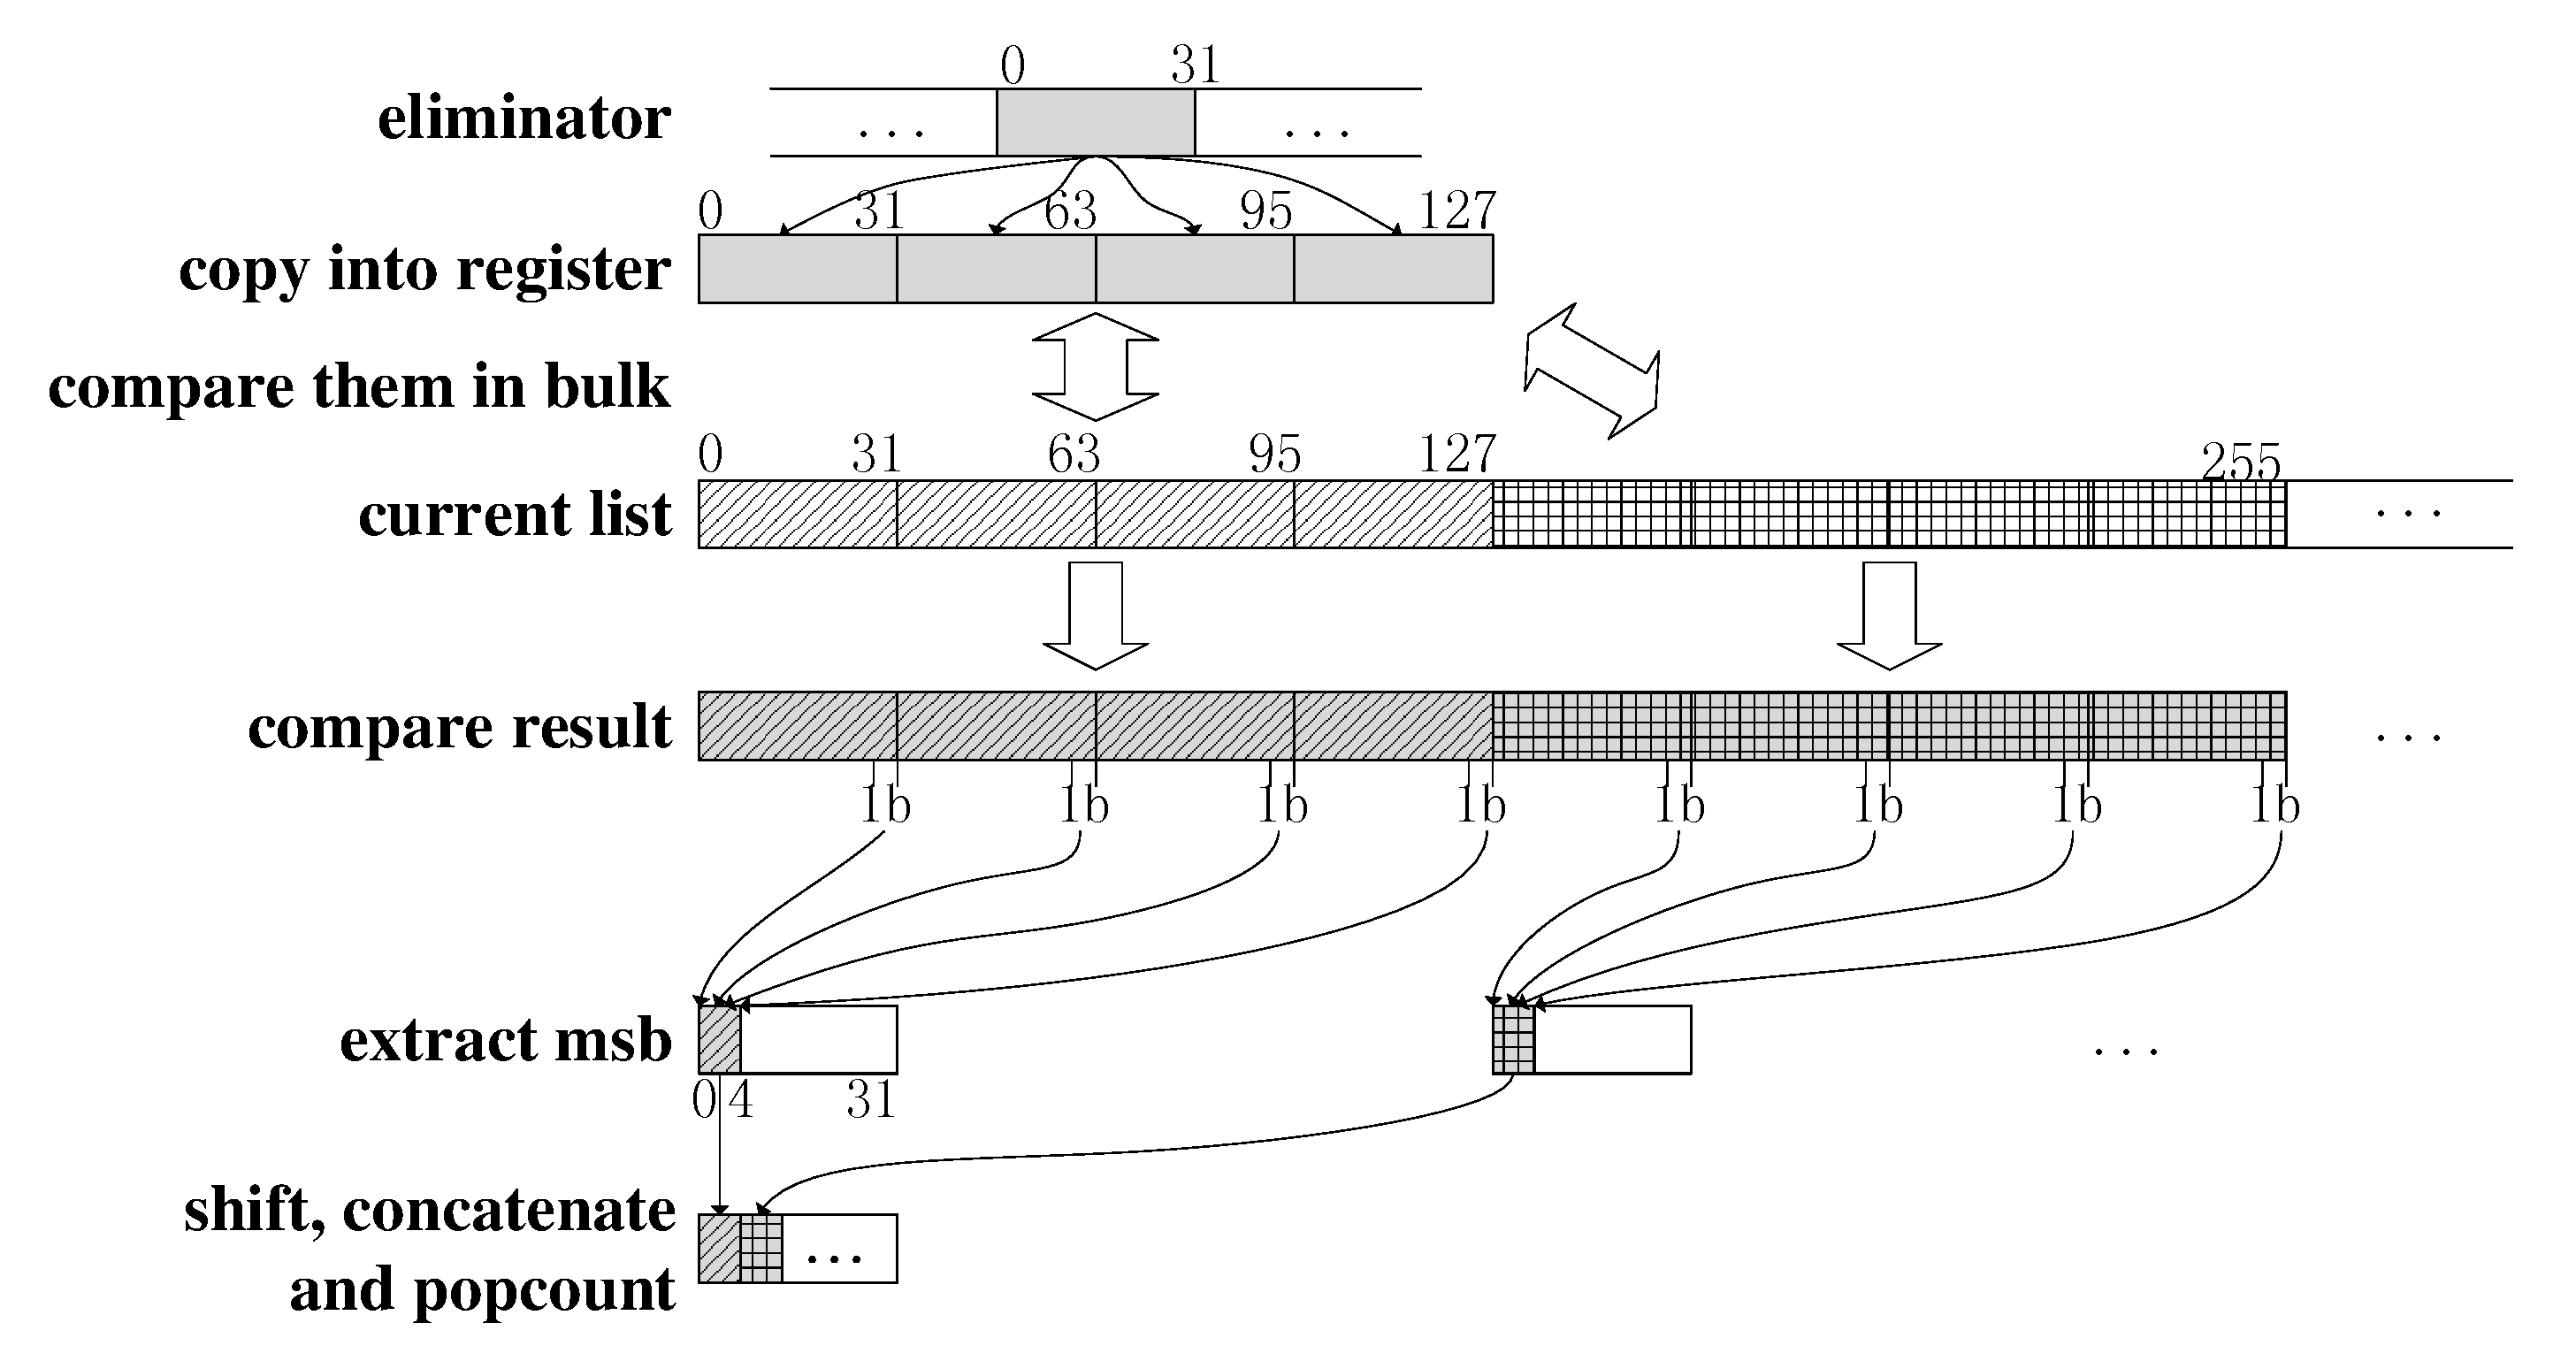
\includegraphics[width=1.0\linewidth]{search}
	\caption{The procedure of our SIMD search algorithm}
	\label{fig: search}
\end{figure}

Since a single word can accommodate at most 32 bits, this scheme is bounded to advance 32 or fewer integers each time ($ w_1 \leq 32 $).
When the set size is large or the matched value is sparse, the whole progress will be delayed by these redundant comparisons.
There two ways to ameliorate this risk.
First, we replace \texttt{PCMPGTD} with more efficient \texttt{PCMPEQD} and omit operations after the comparison.
Namely, return roughly the head position without the exact offset and a flag telling whether a matched value is found, thus $ w_1 $ is not bounded by 32.
With fewer operations, the search efficiency is improved, and the \textit{if\_equal} branch is expected to have fewer mispredictions.
The only cost is repetitive comparisons caused by inexact position, which can be efficiently executed via SIMD instructions.
Second, executing parallel comparison in an element-wise manner falls back to vectorized \texttt{Zipper}.
Before it, a gallop search can be adopted to quickly locate a window $ w_1 $ in which lies a possible match.
Same as SIMD GALLOPING does, given another widow size $ w_2 $, we first sequentially fetch values at $ 1w_2,2w_2,4w_2,\dots $ until a value not less than $ e $ is found, then we bisect current interval to $ w_1 $ to verify the existence via parallel comparison.

Two parameters $ w_1 $ and $ w_2 $ have essential impacts on algorithm's efficiency.
$ w_2 $ represents the skipping rate via scalar \textit{if\_equal} branches, $ w_1 $ represents the primary unit of parallel comparison and the precision of returned position.
In previous work, they are set empirically \cite{inoue2014faster,lemire2016simd}, intuitively, we expect they should vary with the intersecting sets.
We propose a dual-scale search pattern with varying $ (w_1,w_2) $ for optimal efficiency.
In order to quantify the time costs with sufficient accuracy, we first carry out a profiling step of all possible combination $ (w_1,w_2) $, by averaging several runs of intersection on a large artificial data of sorted sets, covering enough scenarios of different size ratios, selectivities and number of sets.
Then from these measurements we learn a predictor that use features extracted from the sets to predict the intersection time.
The predictor is modeled as a linear combination of features with non-negative weights, namely $ t=\textbf{x}^T\textbf{w}+b $, where $ \textbf{w} $ is the feature vector, $ \textbf{w} $ the weights vector and $ b $ the constant bias.
Given a multiset set $ \mathcal{T} = {(x,t)} $ of features and their respective times, we introduce $ L_1 $ loss function to obtain $ \textbf{w}, b $ via linear programming:
\begin{displaymath}
\min_{\textbf{w},b\geq 0} \sum_{(x,t)\in \mathcal{T}}|\textbf{x}^T\textbf{w}+b-t|+\lambda|\mathcal{T}|||\textbf{w}||_1
\end{displaymath}
\noindent where $ \lambda $ is the regularization parameter.
The features chosen are sizes of two currently intersecting sets $ s_1, s_2 $ and $ w_1$, $w_2 $, $\log w_1$, $\log w_2$, $\dfrac{s_2}{w_2}$, $\dfrac{w_2}{w_1} $.
Given a predictor, we can either choose to calculate optimal $ (w_1,w_2) $ on the air, or, more efficiently, build a preprocessed table map to avoid extra cost.
%Thus we are able to choose the optimal $ (w_1,w_2) $ for the input sets.
\section{Experiments}
% use synthetic data rather than real-world data
%As our goal is to find an efficient algorithm for Boolean query in the search engine, and the data is stored as sorted integers in the inverted index.
We choose to use random generated integers to form the sorted sets, in the same way as Baeza Yates and Salinger \cite{Baezayates2005Experimental} and Barbay et al. \cite{barbay2009experimental} did.
Since the crawled data and queries from real world may have some biases, the synthetic data are expected to cover more situations of intersection.
The integers are uniformly distributed in the range $ [0,2^{32}-1] $, the number of sets varies from 2 to 10 by 1.
The smallest size of set keeps doubling from $ 2^{10} $ to $ 2^{14} $, and the size ratio between it and the largest size is set to be $ 1, 10, 10^2, 10^3,$ and $ 10^4 $ respectively, other sizes are assigned randomly between them when the number is larger than 2.
And for each specified configuration of the sets, we generate 50 instances with fixed selectivity (around 40\%), which is consistent with realities.
%
%The sets are generated according to the following steps: we first generate the result set according to selectivity, then all the other sets are created on the basis of the result set to avoid additional intersection, and their sizes are strictly bounded by the predefined smallest and largest sizes.

All the implementations are carried out on a PC server with an 4 core Intel(r) Core(r) i5-4590 processor running at 3.30 GHz, with 16GB RAM and 6MB L3 cache.
Although recent instructions are more powerful to support larger registers (YMM of 256 bits and ZMM of 512 bits), in our experiments we only use 128-bit registers (XMM) to avoid introducing extra performance errors with previous algorithms.
Our algorithm is compiled with G++ 4.8.1 with -O3 optimizations. In all our runs, executions are reported as the mean of 200 consecutive replications.
%%have made substantial efforts applying SIMD instruction to sorted sets intersection.
%However, they only consider intersecting two sets, and for multiple sets they simply imply the task can be done in a \texttt{svs} fashion.
%In realistic Boolean query, we cannot expect the querying sets are always limited to 2.
%And the algorithms by Schlegel and Inoue are more like vectorized \texttt{Zipper}, which suits solely for sets of similar size.
%These methods have not been evaluated for the intersection of multiple sets against the relevant algorithms mention in Sec.~\ref{sec: msis}.
%For the above reasons, in the next sections we provide preliminary experiments on the abovementioned algorithms to test their performance on multiple sets.
%Then we propose our improvements on the .... and analysis on ....
%\section{Preliminary Experiment}
%Before further exploring the optimization on multiple sets intersection, we first declare our data setup, which we also use in the later sections.
%Then we execute preliminary experiments on the algorithms mentioned in Sec.~\ref{sec: msis} to validate their performances on different scenarios.

First we show the performances of the predictor in Figure.~\ref{fig: predictor}.
The average absolute error of our predictor is 80us, which is less than 10\% of the median time in all cases.
From the figure, the predicted time is always than the actual value, for the unpredictable delay caused by branch misprediction and cache miss.
However, the curves show similar tendency along the x-axis, and our is goal is to select optimal $ (w_1,w_2) $ rather than exactly predict the time, the result is acceptable.
Note that this figure only displays average time among all the cases, for the specific situation, the best option differs.
Also notice that for each $ w_2 $ the curve tends to be a concave, namely a large skipping length with a relative small SIMD-comparison window is a better choice.
\begin{figure}
	\centering
	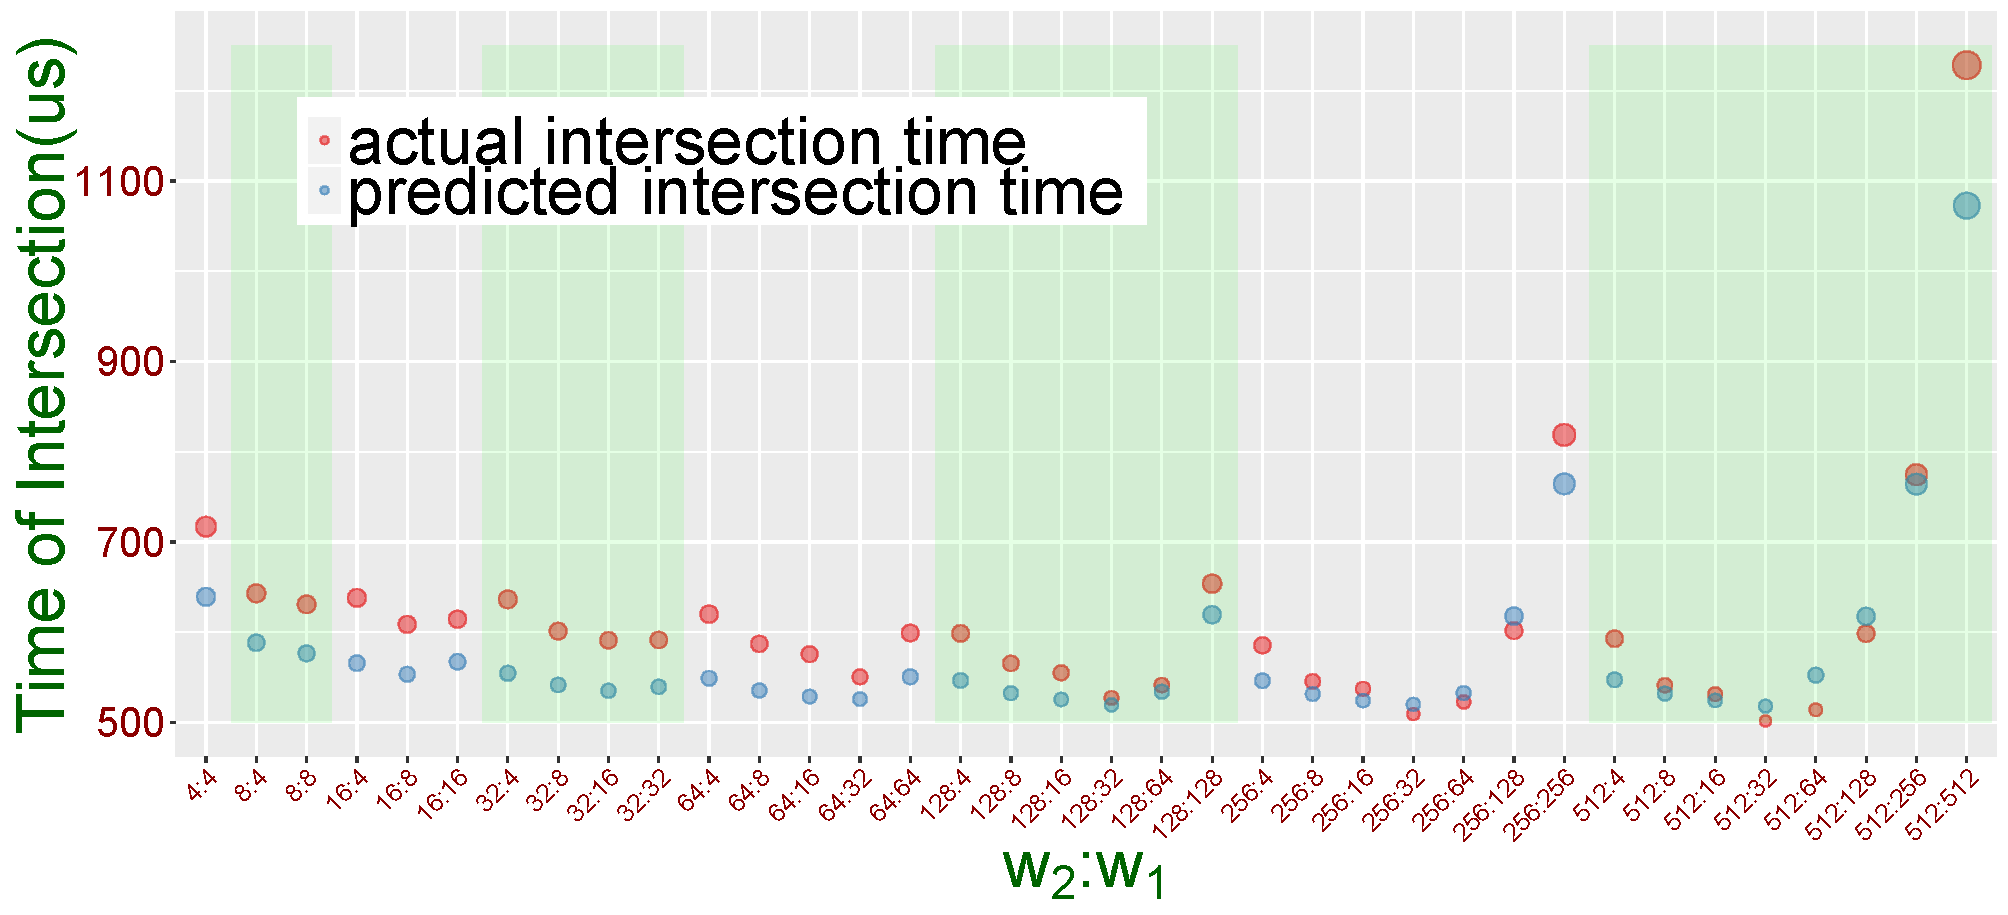
\includegraphics[width=1.0\linewidth]{w2w1}
	\caption{Predicted and actual average intersection times for different $ (w_1,w_2) $. Configurations with same $ w_2 $ are separated using different colour.}
	\label{fig: predictor}
\end{figure}

The proposed dual-scale search algorithm is substituted for the originals of \texttt{max} and SIMD GALLOPING (\texttt{lemire}), called \texttt{max\_opt} and \texttt{svs\_opt}.
For these two methods represent the best efficiency among non-SIMD and SIMD intersection algorithms.
The difference is that \texttt{max\_opt} only uses the predictor once at the beginning while the latter updates $ (w_1,w_2) $ everytime after a set is traversed.

Figure.~\ref{fig: time} shows their performance under different scenarios.
Obviously, time cost grows with the number and size of sets.
Not displayed though selectivity is, we find it barely affects the performance regardless the proportion it accounts.
It is clear that our methods outperform their originals in almost all cases.
When the size ratio is small, \texttt{lemire} performs the best, however, it becomes inferior as the size grow larger, even traditional \texttt{max} overtakes it when size ratio reaches $ 10^4 $.
It also confirms the fact that fixed-sized $ (w_1,w_2) $ can only suit limited scenarios.
On the contrary, \texttt{svs\_opt} maintains a high efficiency among all the methods, validates the effectiveness of the predictor and prove that our dual-scale search algorithm has better performance.
Also worth nothing is that the performance gap between \texttt{max\_opt} and \texttt{svs\_opt} becomes closer as size ratio grows, demonstrating \texttt{max} is suit for large sets intersection.
\begin{figure}
	\centering
	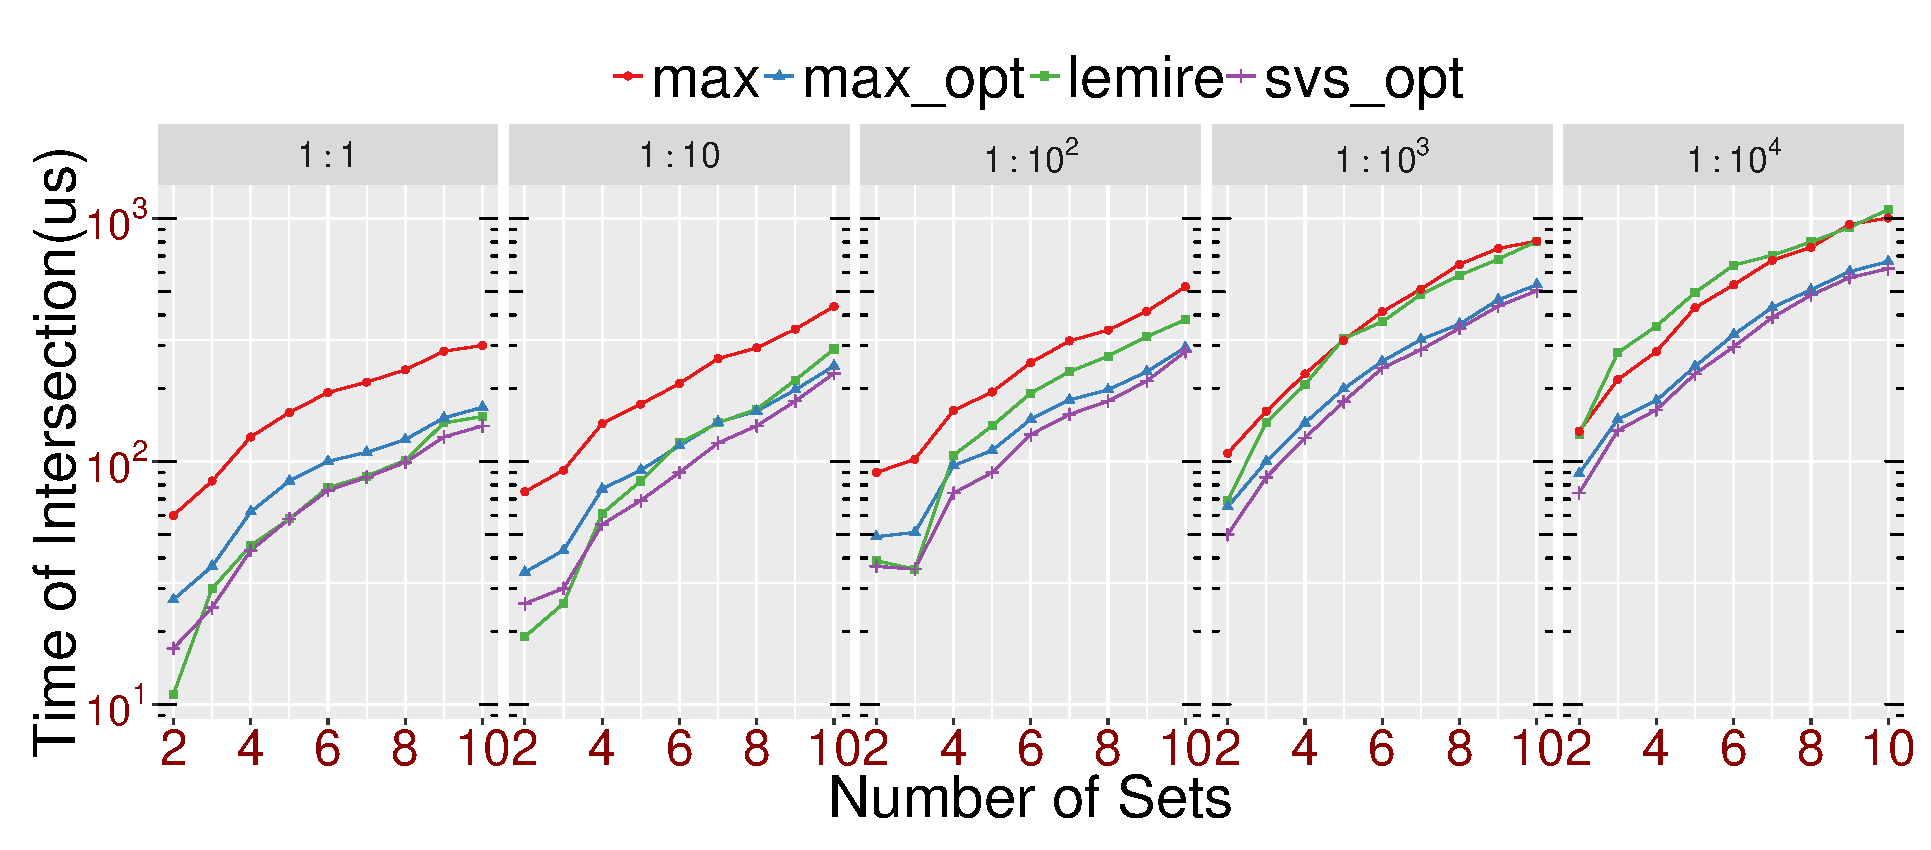
\includegraphics[width=1.0\linewidth]{time}
	\caption{Time cost of optimized intersection algorithms for different set sizes against the original ones. Note the logarithmic scale.}
	\label{fig: time}
\end{figure}

We also give the number distribution of comparisons executed in these SIMD-based algorithms in all cases.
As can be seen in Figure.~\ref{fig: boxplot}, number of comparisons is closely related with the efficiency of algorithms.
Among them, \texttt{svs\_opt} always takes the least comparisons while \texttt{lemire} first outperforms, then falls behind \texttt{max\_opt}.
Notice the huge number gap between 2 and 3, which can be attributed to the fact that sets are less likely to overlap much given a large enough universe.
Numbers tend to grow slowly since invalid values are efficiently eliminated.
\begin{figure}
	\centering
	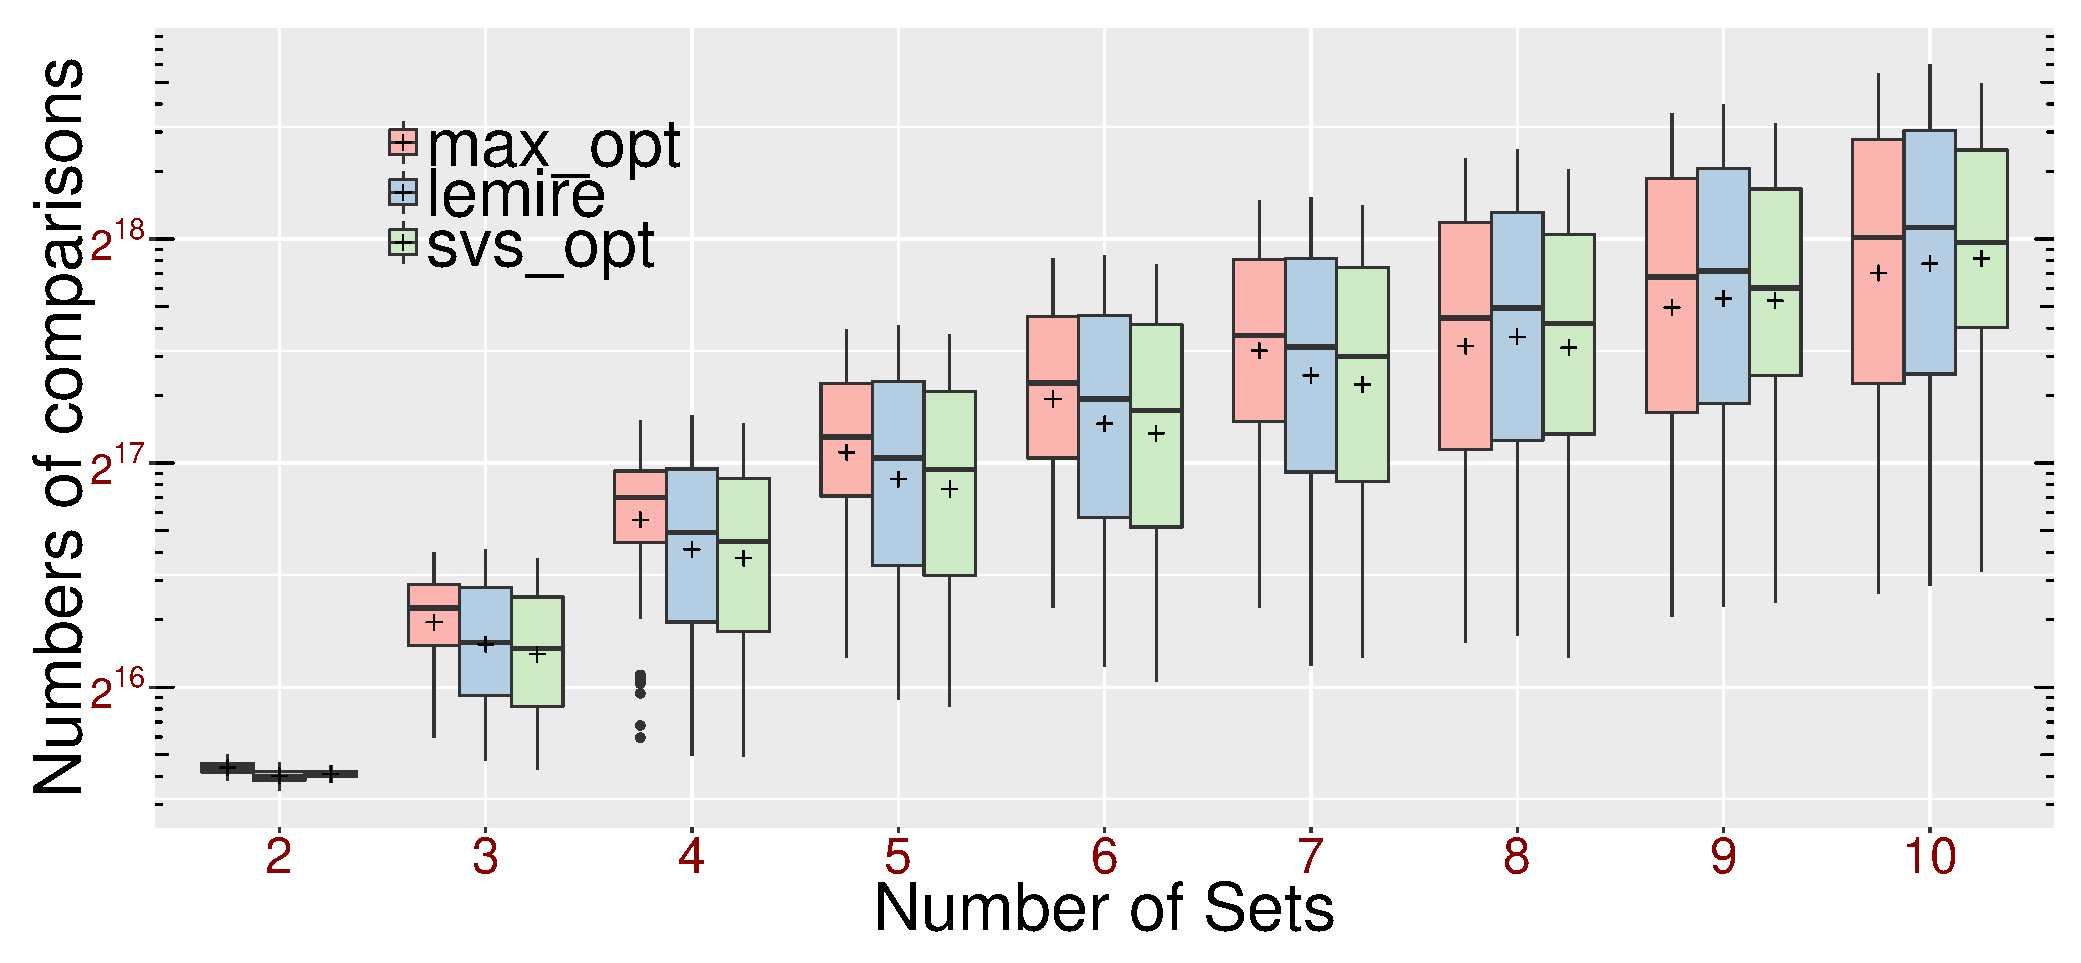
\includegraphics[width=1.0\linewidth]{boxplot}
	\caption{Time cost of optimized intersection algorithms for different set sizes against the original ones. Note the logarithmic scale.}
	\label{fig: boxplot}
\end{figure}

Table.~\ref{tab: proportion} shows the average proportion of comparisons using two different kinds of instructions.
Though three methods stay at a similar level, \texttt{svs\_opt} takes a little higher proportion than the rest two.
And \texttt{max\_opt} takes the least percentage, however, it works better than \texttt{lemire}, owing to its advantage in selecting proper eliminator via non-SIMD comparisons.
\begin{table}
	\caption{proportion of two kinds of comparisons used in each algorithm.}
	\begin{center}
		\renewcommand{\arraystretch}{0.7}
		\setlength\tabcolsep{3pt}
		\begin{tabular}{c*{3}{r}}
			\toprule
			\multirow{2}*{\textsf{type}}& \multicolumn{3}{c}{\textsf{methods}} \\
			\cmidrule(lr){2-4}
			&\texttt{ max\_opt} & \texttt{lemire} & \texttt{svs\_opt} \\
			\midrule
			\textsf{non-SIMD} & 49.6\% & 46.1\% & 40.5\% \\
			\textsf{SIMD} & 50.4\% & 53.9\% & 59.5\% \\
			\bottomrule
			\label{tab: proportion}
		\end{tabular}
	\end{center}
\end{table}

\section{Conclusion}
We have explored parallel comparison via SIMD instructions that can be used to support efficient multiple sets intersection as a contributing factor in the search algorithms.
The proposed dual-scale search algorithm is able to adjust its search windows according to input sets with on additional time costs except a preprocessing to train the predictor.
Also, The low coupling facilitates its adoption in different intersection algorithms.
Experiments show existing intersection algorithms equipped with the proposed method significantly beat the original ones.
As the sets size and number grows larger, the performance gap becomes more obvious.
%\subsection{Dataset and Setup}
%% use synthetic data rather than real-world data
%As our goal is to find an efficient algorithm for Boolean query in the search engine, and the data is stored as sorted integers in the inverted index.
%We choose to use random generated integers to form the sorted sets, in the same way as Baeza Yates and Salinger \cite{Baezayates2005Experimental} and Barbay et al. \cite{barbay2009experimental} did.
%Since the crawled data and queries from real world may have some biases, the synthetic data are expected to cover more situations of intersection.
%The integers are uniformly distributed in the range $ [0,2^{32}-1] $, the number of sets varies from 2 to 10 by 1.
%The smallest size of set keeps doubling from $ 2^{10} $ to $ 2^{14} $, and the size ratio between it and the largest size is set to be $ 1, 10, 10^2, 10^3,$ and $ 10^4 $ respectively, other sizes are assigned randomly between them when the number is larger than 2.
%And for each specified configuration of the sets, we generate three instances of different selectivity: 10\%, 50\% and 100\%.
%
%The sets are generated according to the following steps: we first generate the result set according to selectivity, then all the other sets are created on the basis of the result set to avoid additional intersection, and their sizes are strictly bounded by the predefined smallest and largest sizes.
%
%All the implementations are carried out on a PC server with an 4 core Intel(r) Core(r) i5-4590 processor running at 3.30 GHz, with 16GB RAM and 6MB L3 cache.
%Although recent instructions are more powerful to support larger registers (YMM of 256 bits and ZMM of 512 bits), in our experiments we only use 128-bit registers (XMM) to avoid introducing extra performance errors with previous algorithms.
%Our algorithm is compiled with G++ 4.8.1 with -O3 optimizations. In all our runs, executions are reported as the mean of 200 consecutive replications.
%\subsection{title}
%\begin{figure}
%	\centering
%	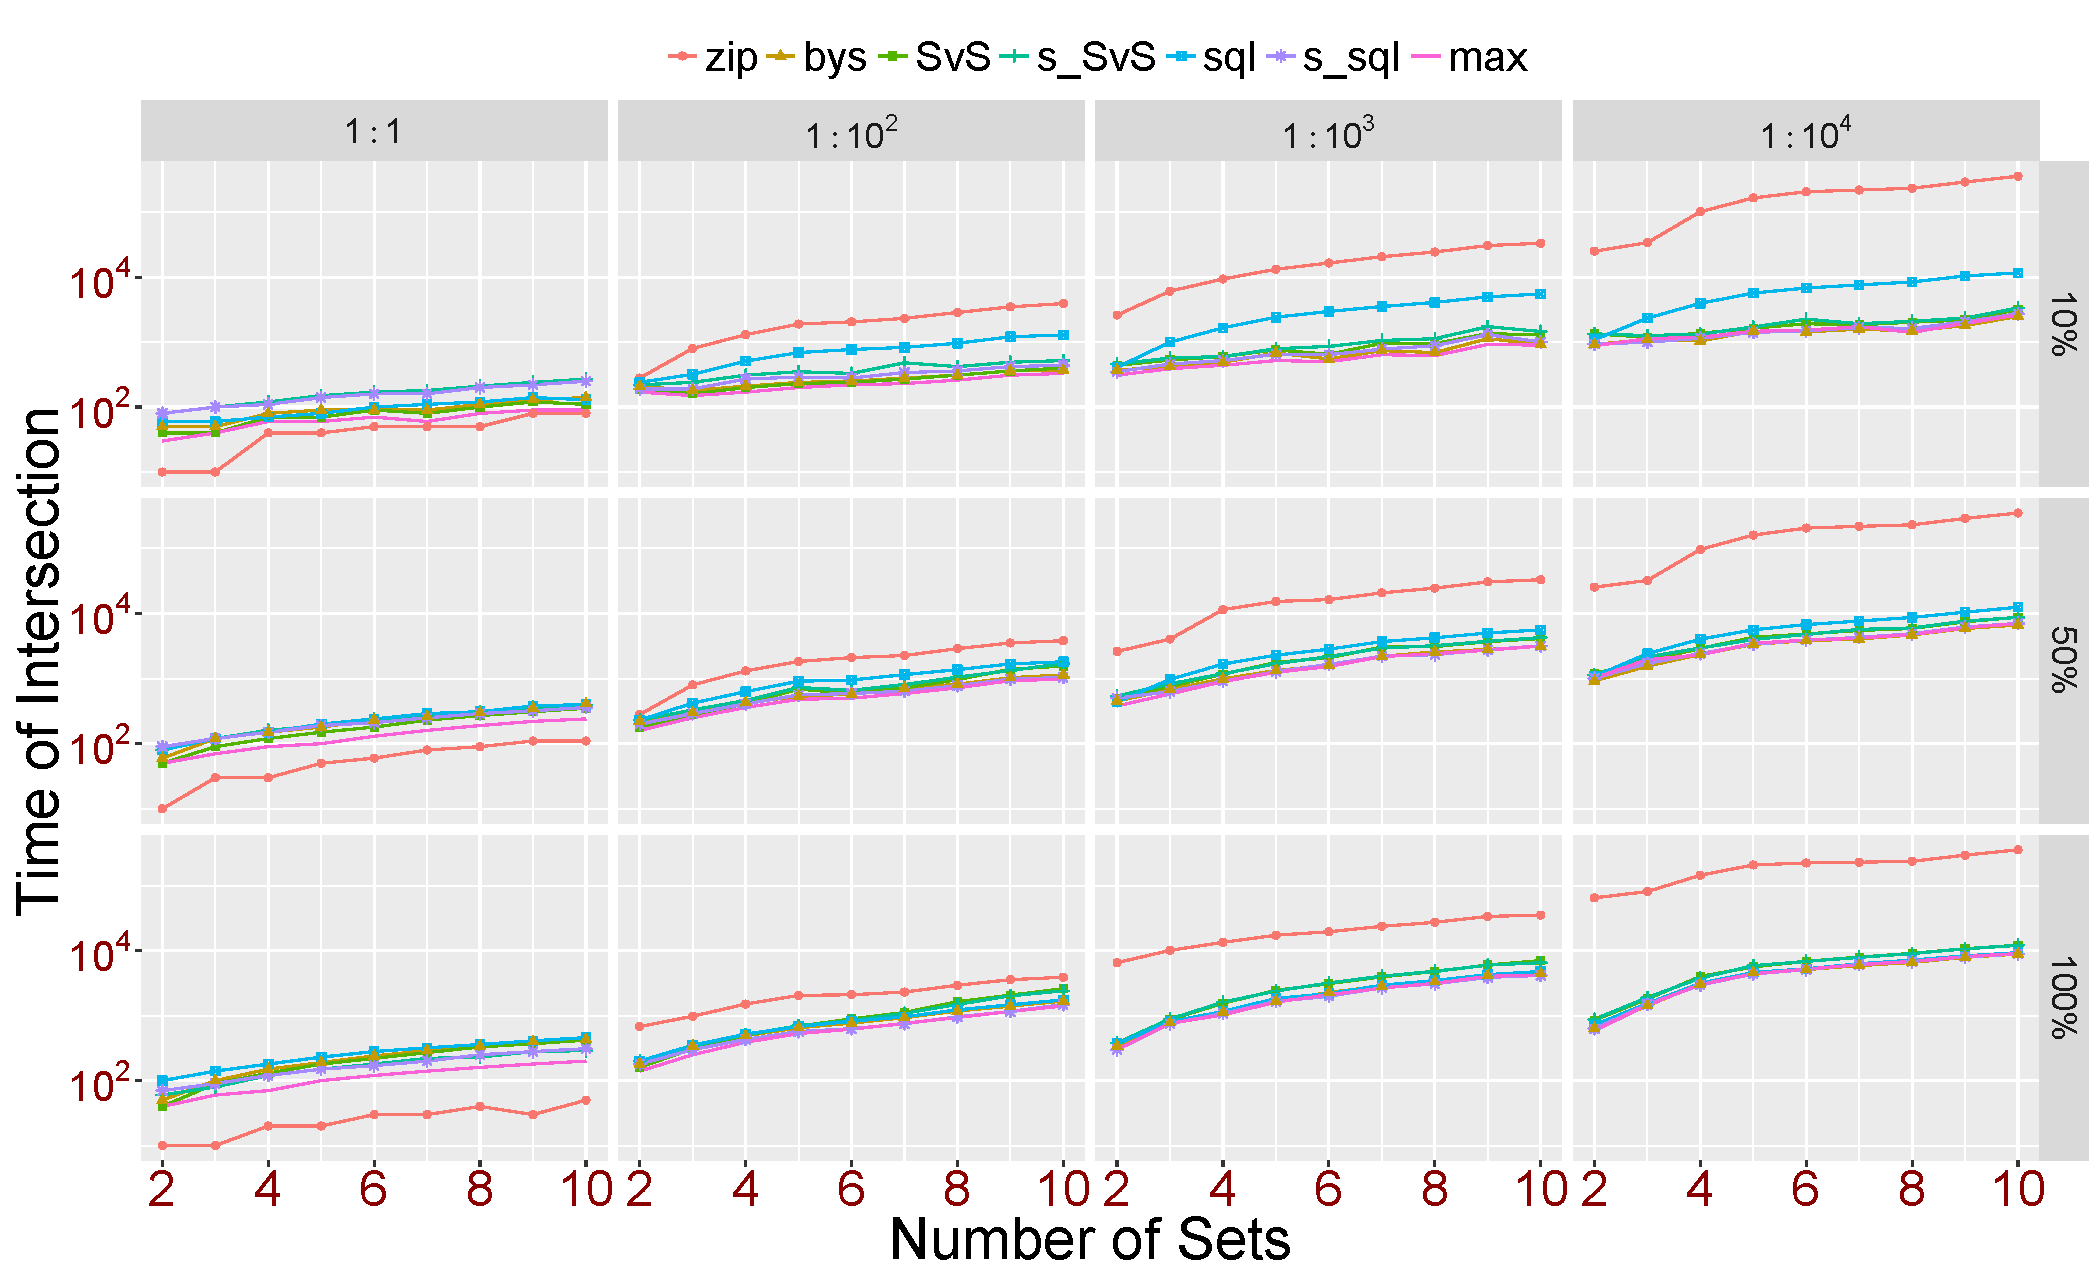
\includegraphics[width=1.0\linewidth]{scalar}
%	\caption{Time cost in microseconds of intersection algorithms under different configurations}
%	\label{fig: scalar}
%\end{figure}
%First we show the Performances of scalar algorithms in Fig.~\ref{fig: scalar}.
%Since \texttt{adp} and \texttt{sql} have few differences and \texttt{sql} always outperforms \texttt{adp} in our experiments,we omit \texttt{adp} and \texttt{s\_adp} and replace them with \texttt{sql} and \texttt{s\_sql} instead.
%Fig.~\ref{fig: scalar} is arranged in two dimensions: rows represent selectivities and columns represent size ratios.
%As can be seen, selectivity hardly affects the performances.
%The overall trend stays nearly the same under different selectivities except that the time cost grows when selectivity becomes larger (Note \texttt{zip} is the only one that achieves faster speed).
%Size ratio plays an important role on the efficiency of different algorithms.
%As the size grows larger, time cost also tends to increase, however, \texttt{zip} performs the best when the size ratio is $ 1:1 $ and the worst in other cases (a more detailed investigation shows it is invincible until $ 1:20 $), demonstrating it only suits for sets of similar size.
%Other algorithms do not differ much from each other, we can see that reordering indeed increases the performance for \texttt{SvS} and \texttt{sql}.
%\texttt{max} is a quite stable method, it performs well in all conditions and \texttt{bys} works better when the size ratio grows larger, it becomes the best one in $ 1:10^4 $.
%Since selectivity hardly distinguishes these algorithms, in the following we only report the performances when selectivity equals 50\% for convenience.
%\begin{figure}
%	\centering
%	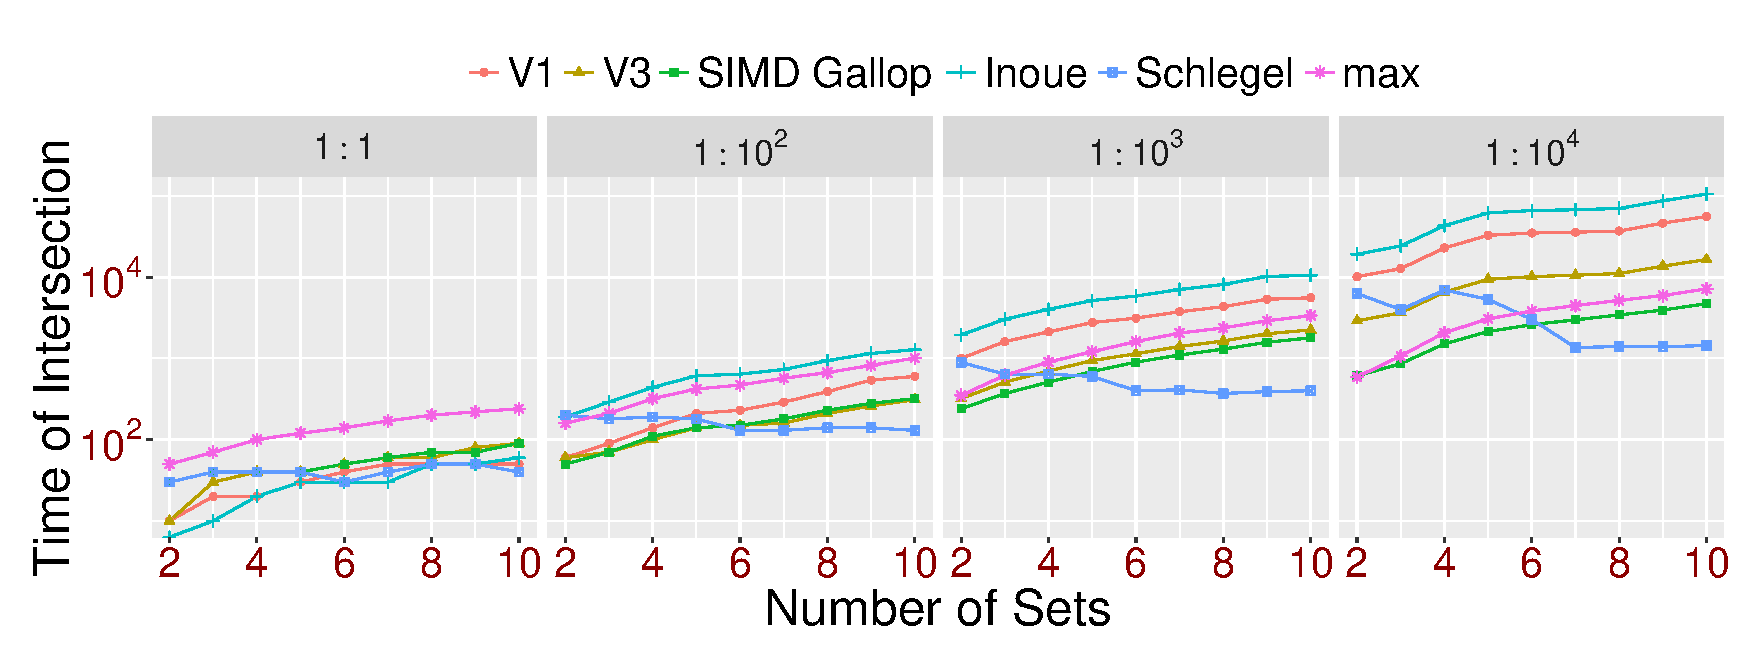
\includegraphics[width=1.0\linewidth]{simd_1}
%	\caption{Time cost in microseconds of SIMD-based intersection algorithms vs. \texttt{max} when selectivity=50\%}
%	\label{fig: simd_1}
%\end{figure}
%
%Fig.~\ref{fig: simd_1} shows the result of the recent SIMD-based algorithms vs. \texttt{max}.
%Specially, sets used for Schlegel have been partitioned to build a hierarchical structure since it only process integers small than $ 2^{16} $.
%As expected, SIMD-based algorithms which work in vectorized \texttt{zip} fashion only performs well when the set sizes are similar.
%In other cases, too many invalid comparisons will sharply slow down their performances and \texttt{max} outperforms them easily.
%On the contrary, SIMD Gallop suits ideally when size ratio grows larger, but only outperforms \texttt{max} by a small margin.
%Performance of Schlegel gets well for multiple sets and large size ratio, the main reason is that it benefits much from the preprocessing.
%The partitioning procedure already compares and sorts the elements inside each sets, and it also takes much time, however, does not taken into account for intersection. 
%\begin{table}
%	\caption[?]{in microseconds.}
%	\begin{center}
%		\renewcommand{\arraystretch}{1}
%		\setlength\tabcolsep{3pt}
%		\begin{tabular}{c*{4}{*{3}rrr}}
%			\toprule
%			\multirow{5}*{\textsf{methods}}& \multicolumn{12}{c}{\textsf{size ratio}} \\
%			\cmidrule(lr){2-13}
%			& \multicolumn{3}{c}{1:1} & \multicolumn{3}{c}{1:$ 10^2 $} & \multicolumn{3}{c}{1:$ 10^3 $} & \multicolumn{3}{c}{1:$ 10^4 $}\\
%			\cmidrule(lr){2-4} \cmidrule(lr){5-7} \cmidrule(lr){8-10} \cmidrule(lr){11-13}
%			& \multicolumn{3}{c}{\textsf{selectivity}} & \multicolumn{3}{c}{\textsf{selectivity}} & \multicolumn{3}{c}{\textsf{selectivity}} & \multicolumn{3}{c}{\textsf{selectivity}}\\ 
%			& 10\% & 50\% & 100\% & 10\% & 50\% & 100\% & 10\% & 50\% & 100\% & 10\% & 50\% & 100\% \\
%			\midrule
%	\texttt{Zipper} &\textbf{45.6} &\textbf{63.3} &\textbf{26.7} &2103.3&2088.9&2228.9&17448.8&17599.9&20806.8&182045.0&178150.1&205375.1\\      
%	\texttt{bys}    &92.2 &228.9&243.3&267.8 &640.0 &846.7 &666.7  &1750.0 &2332.2 &\textbf{1482.2}  &\textbf{3695.6}  &\textbf{4903.4}  \\      
%	\texttt{SvS}    &80.0 &194.4&227.9&262.2 &753.3 &1108.9&836.7  &2248.9 &3352.2 &1854.4  &4741.1  &6570.3  \\      
%	\texttt{s\_SvS} &168.9&235.6&178.9&373.3 &812.2 &1067.8&962.2  &2284.4 &3320.0 &1956.7  &4777.8  &6563.7  \\      
%	\texttt{sql}    &96.7 &241.1&275.6&757.8 &1016.7&886.7 &2953.3 &2971.1 &2427.8 &6448.0  &6573.6  &5157.9  \\      
%	\texttt{s\_sql} &157.8&220.0&182.2&308.9 &610.0 &717.8 &732.2  &1717.8 &\textbf{2180.0} &1564.4  &3866.7  &4945.7  \\      
%	\texttt{max}    &64.4 &138.9&118.9&\textbf{226.7} &\textbf{552.2} &\textbf{688.9} &\textbf{582.2}  &\textbf{1680.0} &2208.9 &1545.6  &3852.2  &4975.7  \\      
%			\bottomrule
%			\label{tab: scalar}
%		\end{tabular}
%	\end{center}
%\end{table} 
%\section{Main Algorithms}
%As we have observed, the recent SIMD-based algorithms have low efficiency on large sets.
%In this section, we would like to introduce our optimization on traditional multiple sets intersection algorithms using SIMD instructions.
%From Sec.~\ref{sec: msis} we know the way to elect eliminator and related searching algorithms are two factors that affect the overall efficiency.
%For now, processors only support loading continuous memory chunks into vector registers.
%Instructions that extract and gather data from separate chunks for each element of the sets are included only by AVX-512VL, which is not available yet \cite{Schlegel2011Fast}.
%So we only consider modifying the searching algorithms, among which Golomb Search and Gallop Search are two methods closely related to vector processing, they 
%% Golomb Search and Gallop Search
%
%\section{Experiments}
%% scalar指令效率比较
%% scalar/vector指令效率比较
%% SIMD分块大小
%% linear/gallop比较
%%% linear search is never a good way to intersection
%% exact/rough/thomas(cmplt/cmpeq)
%% 比较次数统计
%% SIMD指令使用比例
%\section{Conclusions and Future Work}

\bibliographystyle{ACM-Reference-Format}
\bibliography{sigproc,../reference,../reference_intersection} 

\end{document}
